\documentclass[a4paper,10pt]{article}
\usepackage[top=3cm, bottom=3cm, right=4.5cm, left=4.5cm]{geometry}
\usepackage[spanish]{babel}
\usepackage[utf8]{inputenc}
\usepackage[breaklinks=true]{hyperref}
\usepackage{verbatim}
\usepackage{amsmath}
\usepackage{graphicx}
\usepackage{subfig}
\usepackage{float}
%\usepackage{subfigure}
\RequirePackage{fontawesome}
%opening

\begin{document}

\begin{titlepage}
\centering
{
\includegraphics[width=0.9\textwidth]{fing_uncuyo}\par}
\vspace{1cm}
{\bfseries\LARGE Universidad Nacional de Cuyo \par}
\vspace{1cm}
{\scshape\Large Facultad de Ingeniería \par}
\vspace{3cm}
{\scshape\Huge Predicción de Precios de Criptomonedas con ARIMA y Prophet \par}
\vspace{3cm}
{\itshape\Large Proyecto Final: Anexo II\\Inteligencia Artificial I \par}
\vfill
{\Large MOLINA, Mauro \par}
{\Large FLORES, Daniel Emiliano \par}
\vfill
{\Large Marzo 2022 \par}
\end{titlepage}

\newpage

\textbf{\large Gráficos de periodo mensual y semanal aleatorios con ARIMA(2,1,1)}

\begin{figure}[H]
 \centering
  \subfloat[]{
   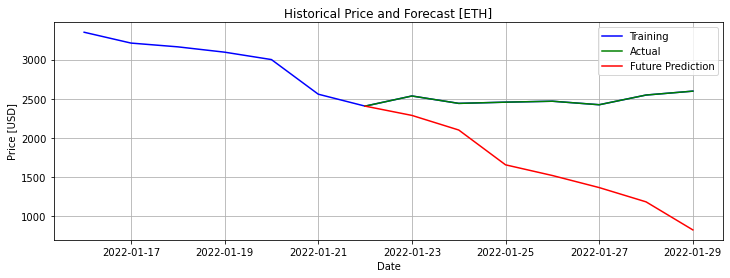
\includegraphics[width=0.5\textwidth]{./plots/arima/plots_eth_random_weekly/eth_wk1}}
  \subfloat[]{
   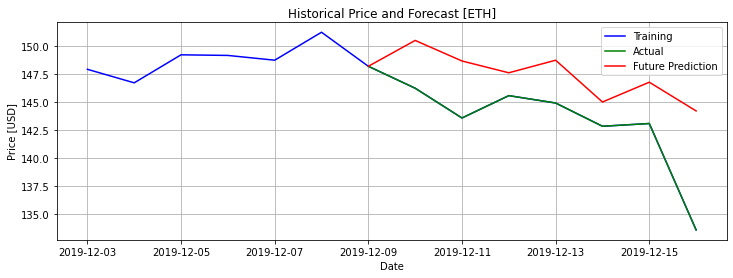
\includegraphics[width=0.5\textwidth]{./plots/arima/plots_eth_random_weekly/eth_wk2}} \\
  \subfloat[]{
   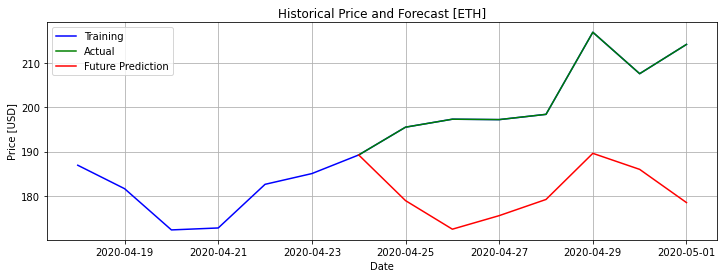
\includegraphics[width=0.5\textwidth]{./plots/arima/plots_eth_random_weekly/eth_wk3}}
   \subfloat[]{
   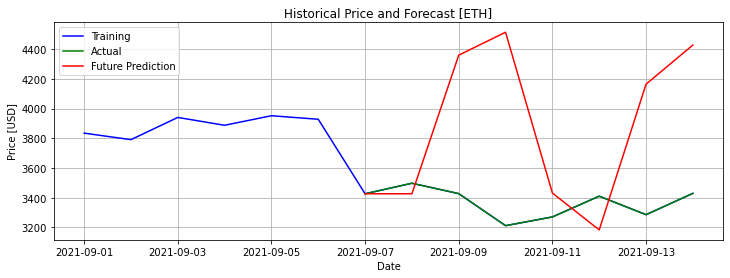
\includegraphics[width=0.5\textwidth]{./plots/arima/plots_eth_random_weekly/eth_wk4}} \\
   \subfloat[]{
   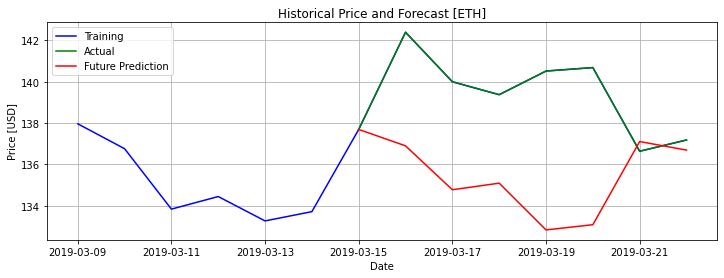
\includegraphics[width=0.5\textwidth]{./plots/arima/plots_eth_random_weekly/eth_wk5}}
   \subfloat[]{
   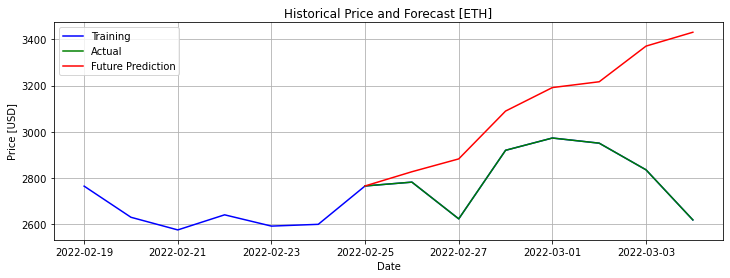
\includegraphics[width=0.5\textwidth]{./plots/arima/plots_eth_random_weekly/eth_wk6}} \\
   \subfloat[]{
   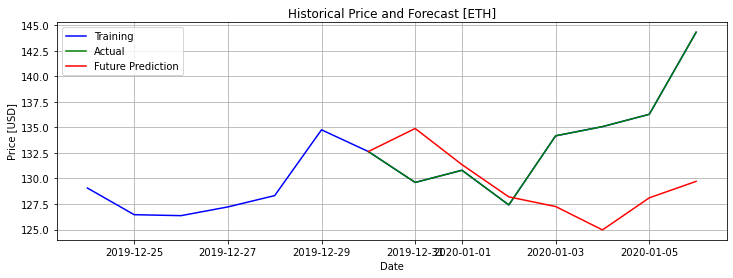
\includegraphics[width=0.5\textwidth]{./plots/arima/plots_eth_random_weekly/eth_wk7}}
   \subfloat[]{
   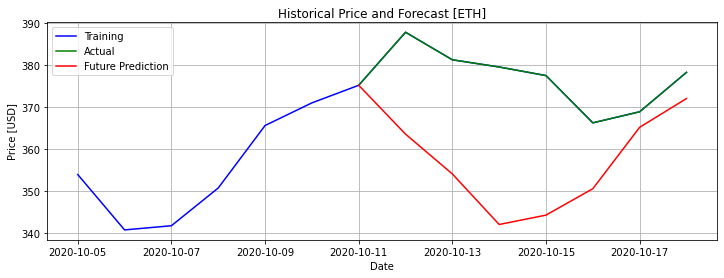
\includegraphics[width=0.5\textwidth]{./plots/arima/plots_eth_random_weekly/eth_wk8}} \\
   \subfloat[]{
   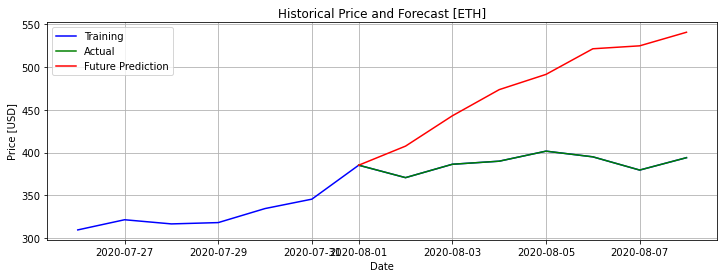
\includegraphics[width=0.5\textwidth]{./plots/arima/plots_eth_random_weekly/eth_wk9}}
   \subfloat[]{
   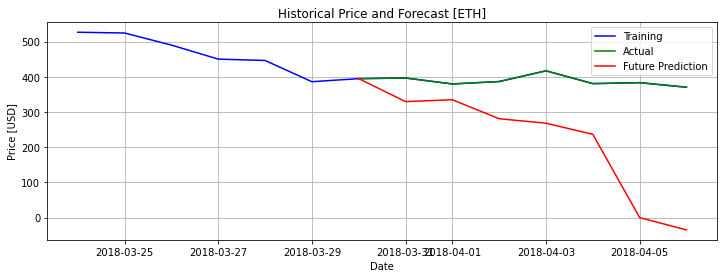
\includegraphics[width=0.5\textwidth]{./plots/arima/plots_eth_random_weekly/eth_wk10}}
  \caption{Predicción del modelo entrenado con 10 semanas aleatorias de ETH}
  \label{f:eth_wk_arima}
\end{figure}

\begin{table}[H]
 \begin{center}
  \begin{tabular}{|r|c|c|c|c|c|c|c|c|c|c|}
    Métrica & (a) & (b) & (c) & (d) & (e) & (f) & (g) & (h) & (i) & (j) \\ \hline
    MAE & 935.3 & 4.528 & 23.87 & 653.4 & 4.467 & 330.2 & 6.628 & 21.04 & 97.74 & 185.6 \\
    RMSE & 1061 & 5.265 & 24.58 & 794.8 & 5.257 & 408.6 & 8.092 & 24.23 & 105.5 & 230.4 \\
    MAPE & 0.372 & 0.032 & 0.116 & 0.196 & 0.032 & 0.119 & 0.048 & 0.055 & 0.251 & 0.484 \\ \hline
  \end{tabular}
  \caption{Métricas de la figura \ref{f:eth_wk_arima}}
  \label{tab:eth}
 \end{center}
\end{table}

\begin{figure}[H]
 \centering
  \subfloat[]{
   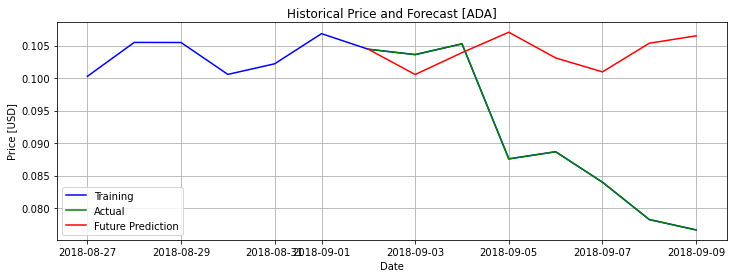
\includegraphics[width=0.5\textwidth]{./plots/arima/plots_ada_random_weekly/ada_wk1}}
  \subfloat[]{
   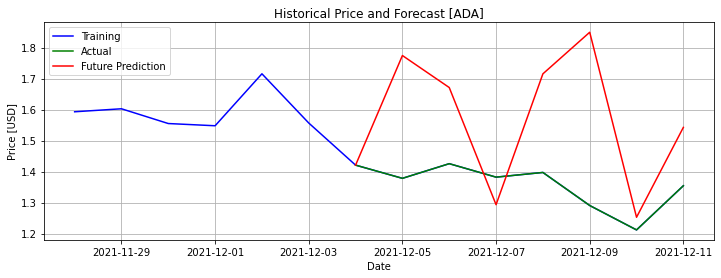
\includegraphics[width=0.5\textwidth]{./plots/arima/plots_ada_random_weekly/ada_wk2}} \\
  \subfloat[]{
   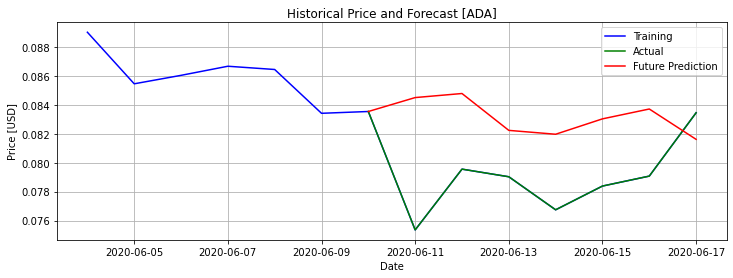
\includegraphics[width=0.5\textwidth]{./plots/arima/plots_ada_random_weekly/ada_wk3}}
   \subfloat[]{
   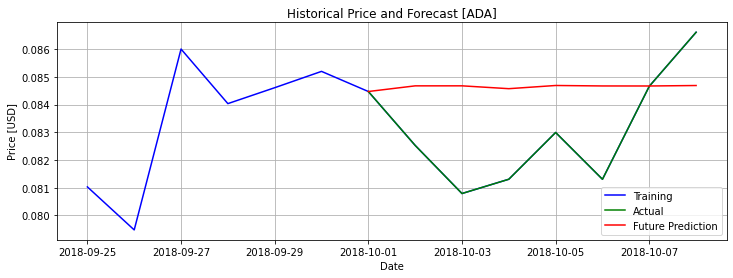
\includegraphics[width=0.5\textwidth]{./plots/arima/plots_ada_random_weekly/ada_wk4}} \\
   \subfloat[]{
   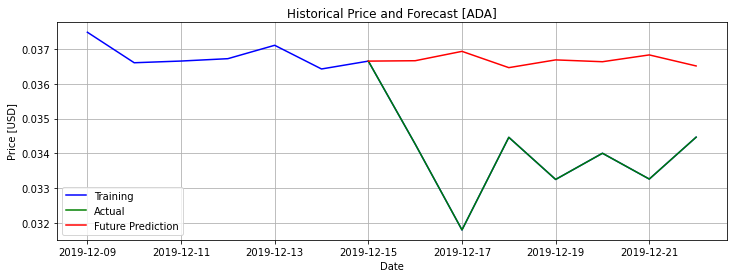
\includegraphics[width=0.5\textwidth]{./plots/arima/plots_ada_random_weekly/ada_wk5}}
   \subfloat[]{
   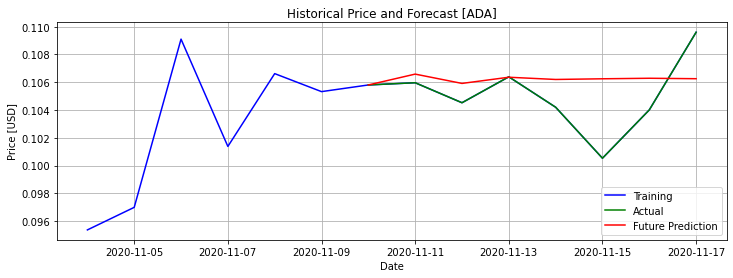
\includegraphics[width=0.5\textwidth]{./plots/arima/plots_ada_random_weekly/ada_wk6}} \\
   \subfloat[]{
   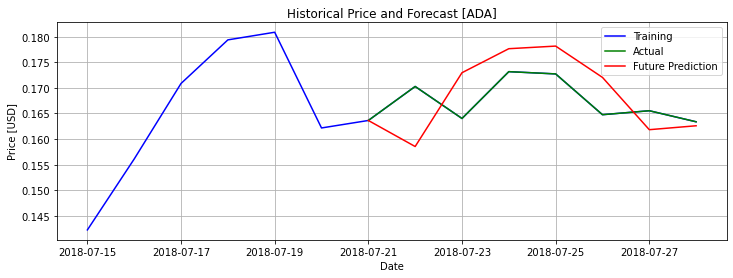
\includegraphics[width=0.5\textwidth]{./plots/arima/plots_ada_random_weekly/ada_wk7}}
   \subfloat[]{
   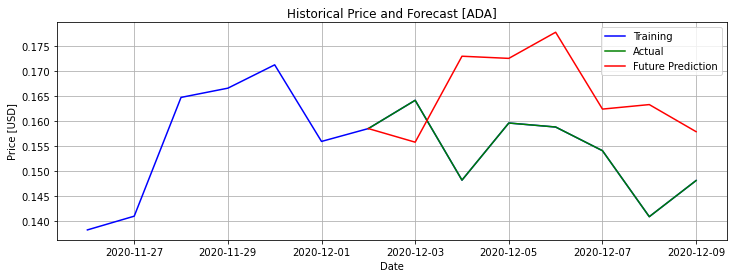
\includegraphics[width=0.5\textwidth]{./plots/arima/plots_ada_random_weekly/ada_wk8}} \\
   \subfloat[]{
   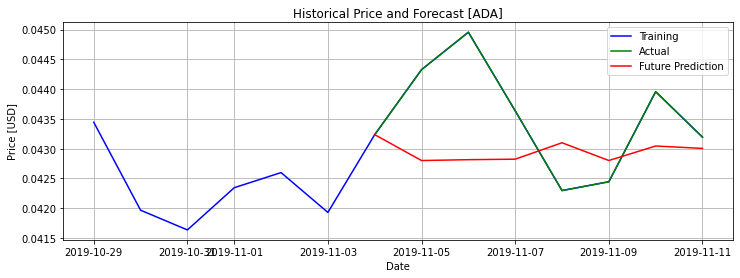
\includegraphics[width=0.5\textwidth]{./plots/arima/plots_ada_random_weekly/ada_wk9}}
   \subfloat[]{
   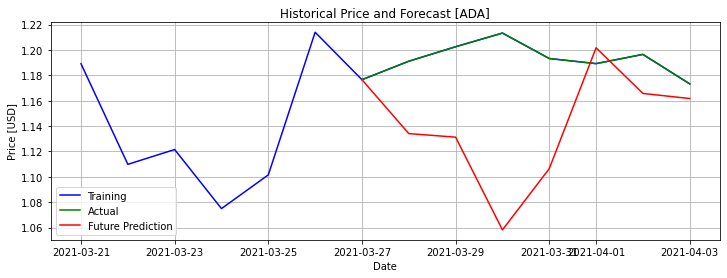
\includegraphics[width=0.5\textwidth]{./plots/arima/plots_ada_random_weekly/ada_wk10}}
  \caption{Predicción del modelo entrenado con 10 semanas aleatorias de ADA}
  \label{f:ada_wk_arima}
\end{figure}

\begin{table}[H]
 \begin{center}
  \begin{tabular}{|r|c|c|c|c|c|c|c|c|c|c|}
    Métrica & (a) & (b) & (c) & (d) & (e) & (f) & (g) & (h) & (i) & (j) \\ \hline
    MAE & 0.016 & 0.262 & 0.004 & 0.002 & 0.003 & 0.002 & 0.006 & 0.015 & 0.001 & 0.061 \\
    RMSE & 0.019 & 0.311 & 0.005 & 0.002 & 0.003 & 0.002 & 0.006 & 0.016 & 0.000 & 0.077 \\
    MAPE & 0.195 & 0.194 & 0.062 & 0.028 & 0.091 & 0.021 & 0.036 & 0.099 & 0.022 & 0.050 \\ \hline
  \end{tabular}
  \caption{Métricas de la figura \ref{f:ada_wk_arima}}
  \label{tab:ada}
 \end{center}
\end{table}

\begin{figure}[H]
 \centering
  \subfloat[]{
   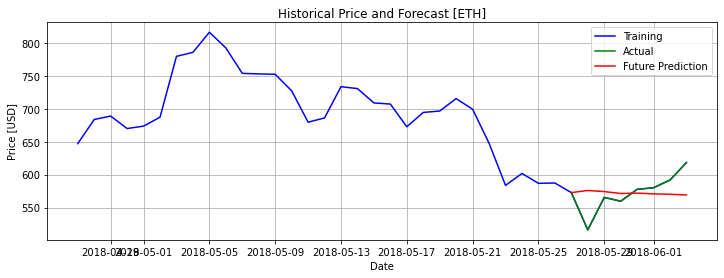
\includegraphics[width=0.5\textwidth]{./plots/arima/plots_eth_random_monthly/eth_mth1}}
  \subfloat[]{
   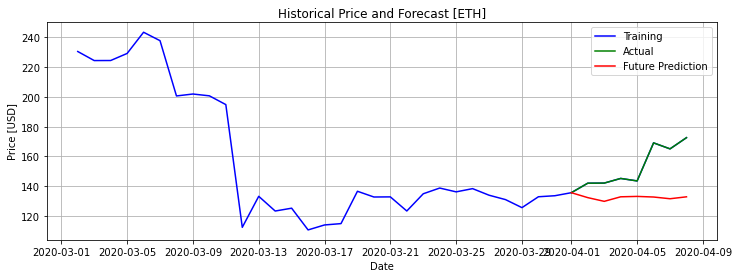
\includegraphics[width=0.5\textwidth]{./plots/arima/plots_eth_random_monthly/eth_mth2}} \\
  \subfloat[]{
   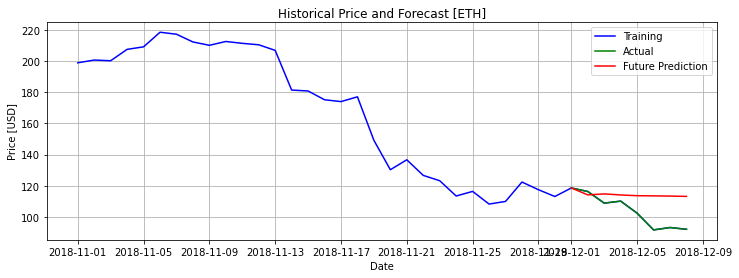
\includegraphics[width=0.5\textwidth]{./plots/arima/plots_eth_random_monthly/eth_mth3}}
   \subfloat[]{
   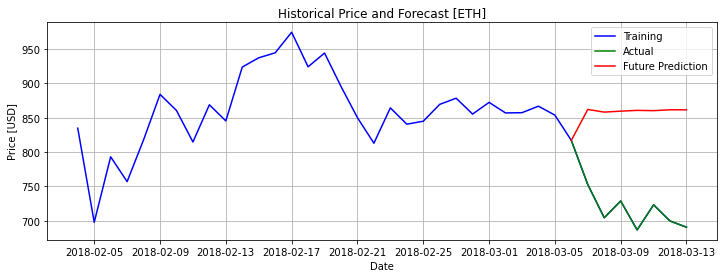
\includegraphics[width=0.5\textwidth]{./plots/arima/plots_eth_random_monthly/eth_mth4}} \\
   \subfloat[]{
   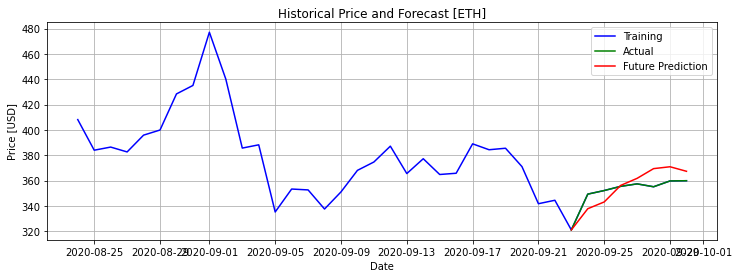
\includegraphics[width=0.5\textwidth]{./plots/arima/plots_eth_random_monthly/eth_mth5}}
   \subfloat[]{
   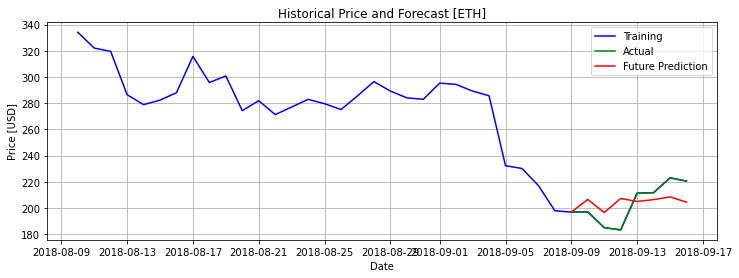
\includegraphics[width=0.5\textwidth]{./plots/arima/plots_eth_random_monthly/eth_mth6}} \\
   \subfloat[]{
   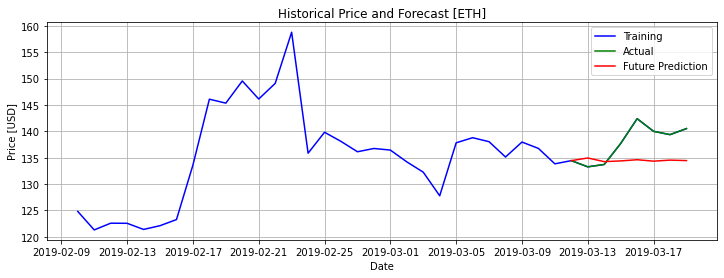
\includegraphics[width=0.5\textwidth]{./plots/arima/plots_eth_random_monthly/eth_mth7}}
   \subfloat[]{
   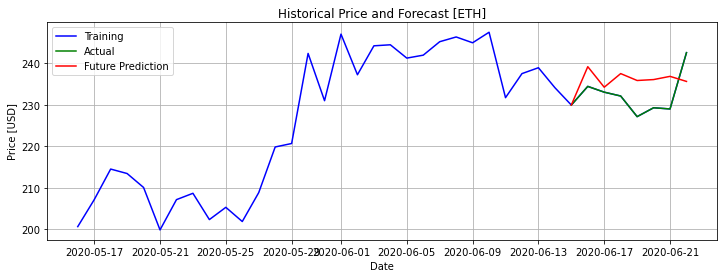
\includegraphics[width=0.5\textwidth]{./plots/arima/plots_eth_random_monthly/eth_mth8}} \\
   \subfloat[]{
   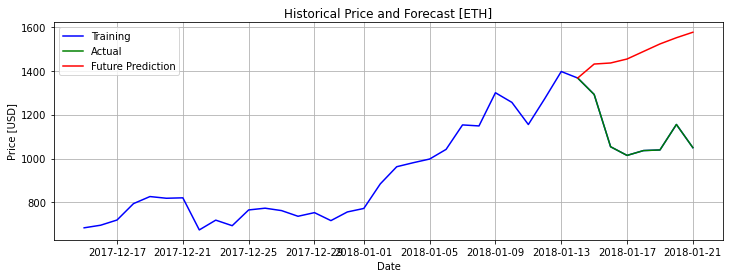
\includegraphics[width=0.5\textwidth]{./plots/arima/plots_eth_random_monthly/eth_mth9}}
   \subfloat[]{
   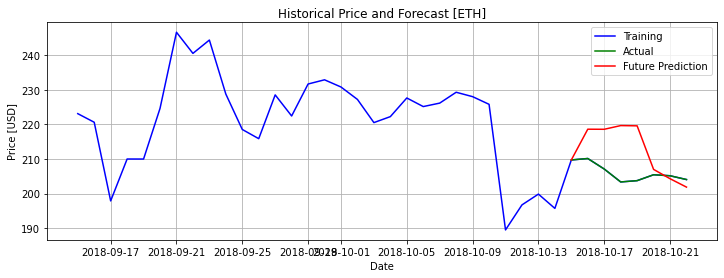
\includegraphics[width=0.5\textwidth]{./plots/arima/plots_eth_random_monthly/eth_mth10}}
  \caption{Predicción del modelo entrenado con 10 meses aleatorios de ETH}
  \label{f:eth_mth_arima}
\end{figure}

\begin{table}[H]
 \begin{center}
  \begin{tabular}{|r|c|c|c|c|c|c|c|c|c|c|}
    Métrica & (a) & (b) & (c) & (d) & (e) & (f) & (g) & (h) & (i) & (j) \\ \hline
    MAE & 23.77 & 22.06 & 12.33 & 147.9 & 8.360 & 12.46 & 4.268 & 5.937 & 402.1 & 8.089 \\
    RMSE & 31.20 & 25.46 & 14.68 & 149.5 & 9.395 & 13.81 & 4.883 & 6.369 & 418.7 & 10.19 \\
    MAPE & 0.042 & 0.137 & 0.129 & 0.209 & 0.023 & 0.062 & 0.030 & 0.026 & 0.378 & 0.039 \\ \hline
  \end{tabular}
  \caption{Métricas de la figura \ref{f:eth_mth_arima}}
  \label{tab:eth_m}
 \end{center}
\end{table}

\begin{figure}[H]
 \centering
  \subfloat[]{
   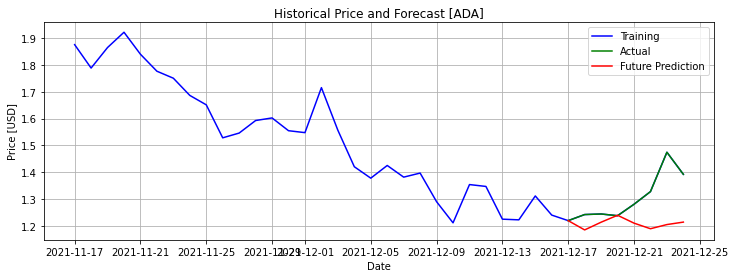
\includegraphics[width=0.5\textwidth]{./plots/arima/plots_ada_random_monthly/ada_mth1}}
  \subfloat[]{
   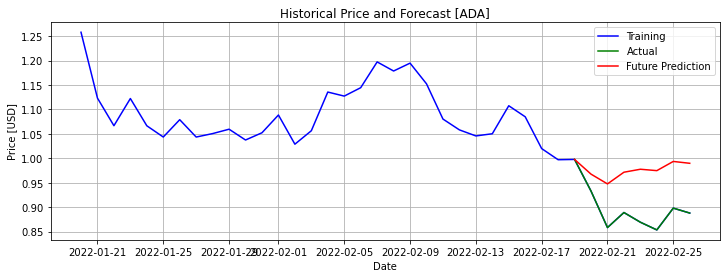
\includegraphics[width=0.5\textwidth]{./plots/arima/plots_ada_random_monthly/ada_mth2}} \\
  \subfloat[]{
   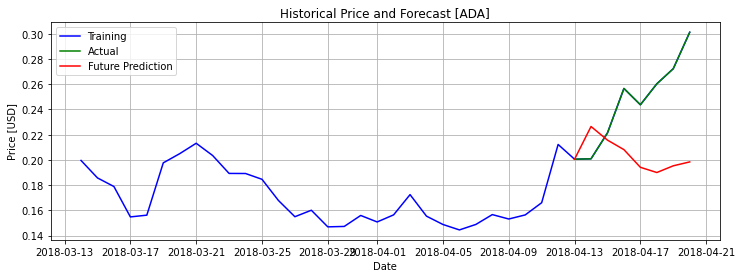
\includegraphics[width=0.5\textwidth]{./plots/arima/plots_ada_random_monthly/ada_mth3}}
   \subfloat[]{
   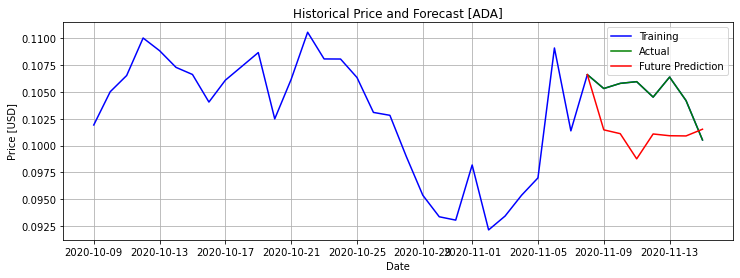
\includegraphics[width=0.5\textwidth]{./plots/arima/plots_ada_random_monthly/ada_mth4}} \\
   \subfloat[]{
   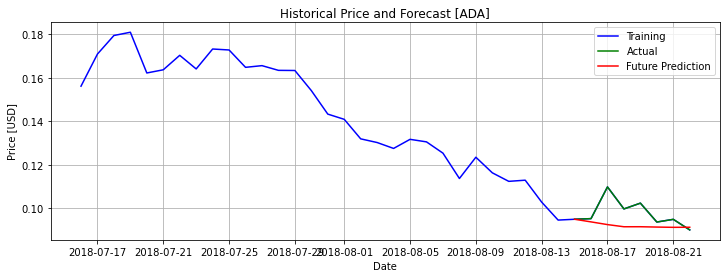
\includegraphics[width=0.5\textwidth]{./plots/arima/plots_ada_random_monthly/ada_mth5}}
   \subfloat[]{
   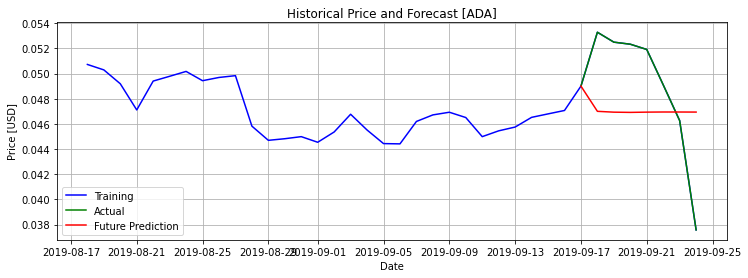
\includegraphics[width=0.5\textwidth]{./plots/arima/plots_ada_random_monthly/ada_mth6}} \\
   \subfloat[]{
   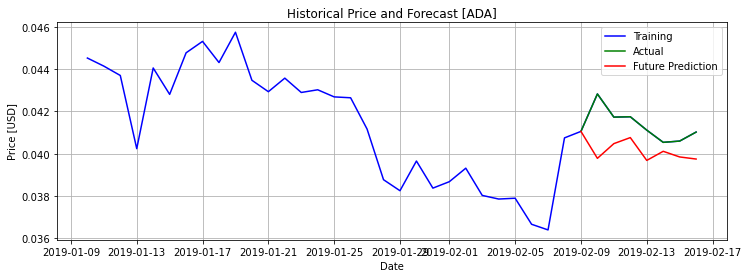
\includegraphics[width=0.5\textwidth]{./plots/arima/plots_ada_random_monthly/ada_mth7}}
   \subfloat[]{
   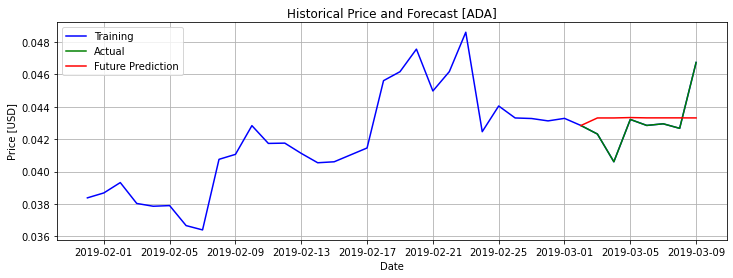
\includegraphics[width=0.5\textwidth]{./plots/arima/plots_ada_random_monthly/ada_mth8}} \\
   \subfloat[]{
   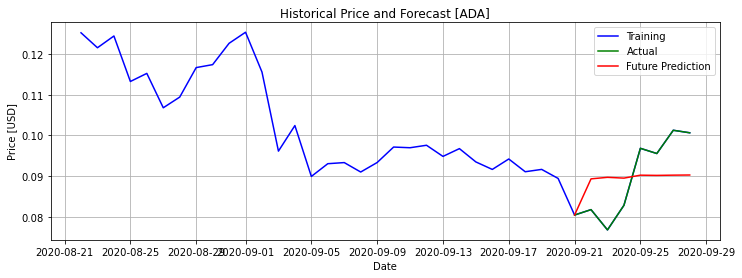
\includegraphics[width=0.5\textwidth]{./plots/arima/plots_ada_random_monthly/ada_mth9}}
   \subfloat[]{
   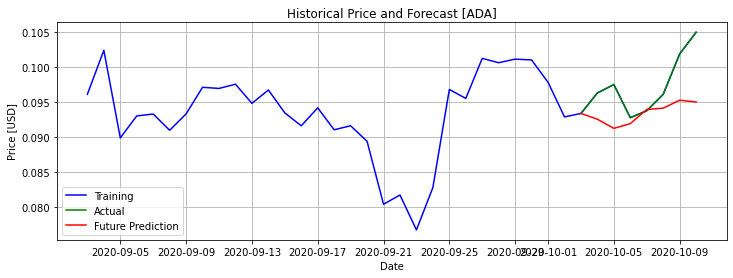
\includegraphics[width=0.5\textwidth]{./plots/arima/plots_ada_random_monthly/ada_mth10}}
  \caption{Predicción del modelo entrenado con 10 meses aleatorios de ADA}
  \label{f:ada_mth_arima}
\end{figure}

\begin{table}[H]
 \begin{center}
  \begin{tabular}{|r|c|c|c|c|c|c|c|c|c|c|}
    Métrica & (a) & (b) & (c) & (d) & (e) & (f) & (g) & (h) & (i) & (j) \\ \hline
    MAE & 0.106 & 0.090 & 0.054 & 0.004 & 0.006 & 0.004 & 0.001 & 0.001 & 0.009 & 0.004 \\
    RMSE & 0.137 & 0.094 & 0.062 & 0.004 & 0.008 & 0.005 & 0.001 & 0.002 & 0.009 & 0.004\\
    MAPE & 0.077 & 0.103 & 0.205 & 0.039 & 0.062 & 0.104 & 0.031 & 0.028 & 0.096 & 0.042 \\ \hline
  \end{tabular}
  \caption{Métricas de la figura \ref{f:ada_mth_arima}}
  \label{tab:ada_m}
 \end{center}
\end{table}

\end{document}
